\section{Working through Dysthe's stability calculation}
\label{sec:stability}
\subsection{Linearization about a uniform nonlinear wavetrain}
The uniform solution remains \eqref{eq:plane-wave}, with zero induced mean
current and elevation. Use \eqref{eq:perturbation}; Dysthe's $a',\theta'$
are our $\eta u,\eta v$. In this section the common factor $\eta$ is
suppressed, and the mean perturbation is first order in $\eta$.

Starting from the paper's printed equations (3.2)--(3.3), independently of
the discrepancy noted in Section~\ref{sec:source-consistency}, gives
\begin{align}
 P_1u+\frac14A_0^2u_x+P_2v&=-\frac12\Ph_z,
 \label{eq:dysthe-linear-a}\\
 P_1v+\frac74A_0^2v_x-P_2u+A_0^2u&=-\frac12\Ph_x,
 \label{eq:dysthe-linear-b}
\end{align}
where
\[
 P_1=\partial_t+\frac12\partial_x
 +\frac1{16}(6\partial_x\partial_y^2-\partial_x^3),
 \qquad P_2=\frac14\partial_y^2-\frac18\partial_x^2.
\]
The mean boundary condition linearizes as
\begin{equation}\label{eq:mean-linearized}
 \Ph_z=2A_0^2u_x,
\end{equation}
because $|A|^2=A_0^2(1+2\eta u)+O(\eta^2)$.

The extra $u_x$ term in \eqref{eq:dysthe-linear-a} changes from $1/4$ to
$5/4$ when its right side is moved left using \eqref{eq:mean-linearized}.

\subsection{Eliminate the mean field using the half-space solution}
For the mode $e^{i(\lambda x+\mu y-\Omega t)}$ with $K>0$,
\[
 \widehat{\Ph}(z)=\frac{2i\lambda A_0^2}{K}\widehat u\,e^{Kz},
 \qquad
 \widehat{\Ph_x}(0)=-\frac{2\lambda^2A_0^2}{K}\widehat u.
\]
Define the quantities used in the paper:
\begin{equation}\label{eq:Pbars}
 \Ps=\Omega-\frac\lambda2+\frac{\lambda}{16}(6\mu^2-\lambda^2),
 \qquad \Pt=\frac{\lambda^2}{8}-\frac{\mu^2}{4}.
\end{equation}
$P_1$ acts as $-i\Ps$, while $P_2$ acts as $\Pt$.
The bar in these two symbols is a paper convention for the algebraic
quantities, not a time average of the operators.

The two perturbation equations become
\begin{equation}\label{eq:dysthe-matrix}
 \begin{pmatrix}
 -i(\Ps-\frac54\lambda A_0^2)&\Pt\\
 A_0^2(1-\lambda^2/K)-\Pt&-i(\Ps-\frac74\lambda A_0^2)
 \end{pmatrix}
 \begin{pmatrix}\widehat u\\\widehat v\end{pmatrix}=0.
\end{equation}
Taking the determinant recovers (3.6):
\begin{equation}\label{eq:dysthe-det}
 (\Ps-\tfrac54\lambda A_0^2)(\Ps-\tfrac74\lambda A_0^2)
 =\Pt\{\Pt-A_0^2(1-\lambda^2/K)\}.
\end{equation}
The mean current modifies the effective nonlinear factor by
$1-\lambda^2/K$. Its dependence on modulation wavenumber is essential.

\subsection{Why the paper discards a term after solving the quadratic}
Completing the square gives the exact roots of this truncated determinant:
\begin{equation}\label{eq:exact-root-truncated}
 \Ps=\frac32\lambda A_0^2
 \mathbin{\pm}
 \sqrt{\Pt\{\Pt-A_0^2(1-\lambda^2/K)\}
              +\frac1{16}\lambda^2A_0^4}.
\end{equation}
But $A_0,\lambda,\mu=O(\varepsilon)$, so $\Pt=O(\varepsilon^2)$.
The radicand contains a leading fourth-order term and a fifth-order
mean-current correction. The added $\lambda^2A_0^4/16$ is sixth order.
Other contributions of that order could come from fifth-order terms
omitted from the original envelope equation. Retaining this one term
would not supply a consistently more accurate physical prediction.

Dysthe therefore uses the asymptotically consistent root (3.7):
\begin{equation}\label{eq:consistent-root}
 \Ps\simeq\frac32\lambda A_0^2
 \mathbin{\pm}\sqrt{\Pt\{\Pt-A_0^2(1-\lambda^2/K)\}}.
\end{equation}
Here $\simeq$ explicitly indicates truncation. Away from marginal roots,
the discarded sixth-order radicand term changes the frequency at fourth
order, beyond the third-order frequency correction supported by the
fourth-order field equation. Near a zero radicand, such square-root
expansions need extra care; do not claim a uniform error estimate there.

The real offset in \eqref{eq:Pbars} contains the higher linear dispersion;
$3\lambda A_0^2/2$ is also real. They shift mode frequency but do not
alter its imaginary part at this order. The growth-rate change is traced
to the horizontal induced current.

\subsection{Longitudinal instability band}
For $\mu=0$, $K=|\lambda|$, so the growing root has
\begin{equation}\label{eq:dysthe-growth}
 \gamma^2=\frac{\lambda^2}{8}
 \left[A_0^2(1-|\lambda|)-\frac{\lambda^2}{8}\right].
\end{equation}
Within the narrowband regime, the exponential instability condition is
\begin{equation}\label{eq:dysthe-band}
 0<\lambda^2<8A_0^2(1-|\lambda|).
\end{equation}
The explicit exclusion of $\lambda=0$ means that the uniform perturbation
has zero exponential growth. It is a neutral symmetry mode, not a growing
sideband.

For $\lambda>0$, solving the approximate marginal condition gives
\[
 \lambda_c=-4A_0^2+\sqrt{8A_0^2+16A_0^4}
           =2\sqrt2A_0-4A_0^2+O(A_0^3).
\]
This closed form is exact for the displayed approximate band equation,
not an all-orders water-wave stability boundary.

The real frequency from the full retained root is
\[
 \operatorname{Re}\Omega=\frac\lambda2+\frac{\lambda^3}{16}
                         +\frac32\lambda A_0^2
 \qquad(\mu=0,\ \gamma>0).
\]
At the marginal mode, retaining through $A_0^2$ gives
\begin{equation}\label{eq:marginal-frequency}
 \Omega_c\simeq\sqrt2A_0(1-\sqrt2A_0),
\end{equation}
which is Dysthe (3.9). Higher-order frequency terms require a
correspondingly higher-order determination of the cutoff.

\subsection{Find the fastest growing mode}
Set $s=A_0>0$ and use $\lambda>0$. Differentiate
\eqref{eq:dysthe-growth}:
\[
 \gamma^2=\frac{s^2\lambda^2}{8}
          -\frac{s^2\lambda^3}{8}-\frac{\lambda^4}{64},
 \qquad
 \frac{\rad\gamma^2}{\rad\lambda}
 =\frac\lambda{16}(4s^2-6s^2\lambda-\lambda^2).
\]
The positive stationary root is
$\lambda_M=-3s^2+\sqrt{4s^2+9s^4}$. Expand at small $s$:
\begin{equation}\label{eq:lambda-max}
 \lambda_M=2s-3s^2+O(s^3).
\end{equation}
Substitution into the growth formula gives
$\gamma_M^2=s^4/4-s^5+O(s^6)$ and hence
\begin{equation}\label{eq:gamma-max}
 \gamma_M=\frac12s^2(1-2s)+O(s^4).
\end{equation}
Finally, substituting \eqref{eq:lambda-max} into the real frequency and
retaining through $s^2$ gives
\begin{equation}\label{eq:frequency-max}
 \operatorname{Re}\Omega_M=s(1-\tfrac32s)+O(s^3).
\end{equation}
These are (3.10)--(3.12). The mode and maximum-growth corrections have
different absolute orders because the leading quantities have different
orders. The approximate formula at $s=0.5$ must not be interpreted as an
established complete stabilization threshold.

\begin{figure}[htbp]
\centering
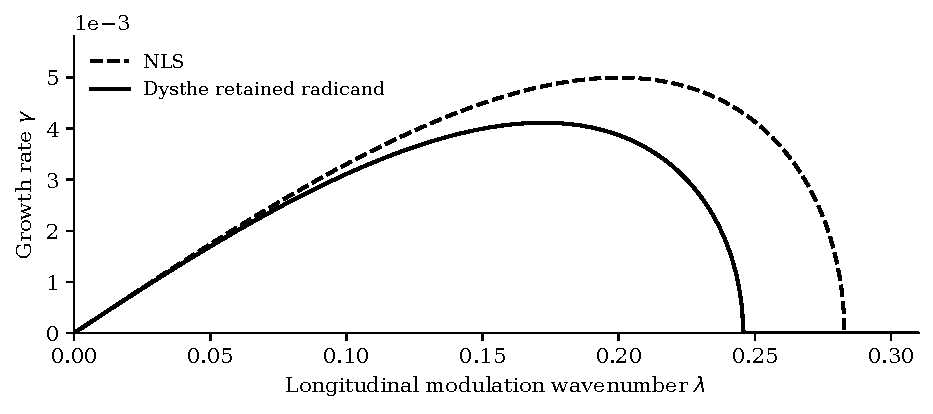
\includegraphics[width=\linewidth]{figures/longitudinal-growth.pdf}
\caption{Growth rates from the NLS radicand and Dysthe's consistently
truncated radicand, for illustrative $A_0=0.10$. These curves compare
reduced formulas; no full-equation or experimental data are included.}
\label{fig:growth}
\end{figure}

\subsection{Transverse modulations and the paper's figures}
For general $\lambda,\mu$, the retained growing root is
\begin{equation}\label{eq:oblique-growth}
 \gamma=\sqrt{[A_0^2(1-\lambda^2/K)-\Pt]\Pt},
\end{equation}
where the radicand must be positive and the wavevector must lie in the
slow-modulation regime. For small $K$, the effective nonlinear factor is
positive, so instability requires
$0<\Pt<A_0^2(1-\lambda^2/K)$.
The current correction depends on the direction of the modulation as
well as its size. Dysthe finds the largest retained growth for $\mu=0$,
removing the unbounded maximum-growth hyperbola of NLS.

The paper also discusses a formal large-$K$ cutoff near $3/2$, and
explicitly notes that this is outside the model's validity range.
Do not turn that formal feature into a physical cutoff theorem.

\begin{figure}[htbp]
\centering
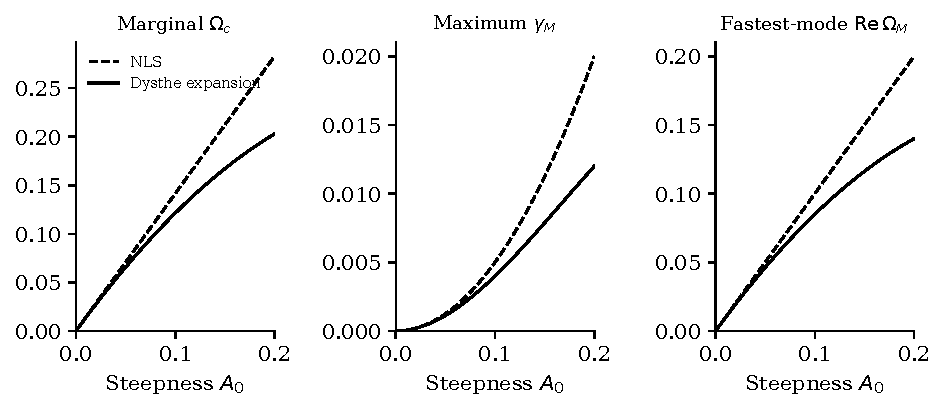
\includegraphics[width=\linewidth]{figures/asymptotic-comparison.pdf}
\caption{The leading NLS formulas and the small-steepness corrections
(3.9), (3.10), and (3.12), plotted only to $A_0=0.20$ for illustration.
The full-equation and laboratory curves in Dysthe's original figures are
not reproduced.}\label{fig:comparison}
\end{figure}

Read the original figures as follows. Figure~1 plots the modulation
frequency at marginal stability, not the carrier frequency.
Figure~2 plots the maximum exponential growth rate.
Figure~3 plots the real frequency separation of the fastest growing
sideband, not its growth rate. The paper reports especially good
agreement of (3.9)--(3.10) with its reference calculations below steepness
roughly $0.3$, while (3.12) underestimates the frequency shift above roughly
$0.2$. These are observable-specific comparisons, not a guarantee of
accuracy for every packet throughout that range.

\paperlink{Read (3.1)--(3.13), printed pp.~110--113. Follow
\eqref{eq:dysthe-matrix} to \eqref{eq:consistent-root}, then compare each
of the three original figure axes with the corresponding formula.}
\checkpoint{Complete the square in \eqref{eq:dysthe-det} and explain
why its exact algebraic root is not a higher-order physical result.}
\clearpage
